\documentclass[
    12pt, % Schriftgröße
    oneside, % zweiseitiger Modus
    ngerman, % deutsches Dokument
    BCOR=0mm, % Bindungskorrektur
    DIV=10 % Division (Anzahl Spalten/Zeilen pro Seite, bestimmt implizit Margins)
]{scrreprt}

\newcommand{\titleDocument}{COBOL}
\newcommand{\authorDocument}{Leon Jarosch}
\newcommand{\subjectDocument}{Abgabeübung}
\newcommand{\locationDocument}{Köln}
\newcommand{\dateDocument}{\today} % Alternativ z.B. 30.~September 2021

\title{\titleDocument}
\author{\authorDocument}
\date{\dateDocument}

\usepackage{dokumentation}

\begin{document}
    % ============ Anfang =============
    % Titelseite
    \include{title}

    % Eidesstattliche Erklärung und Abstrakt
%    \begingroup
    % keine Seitenzahl und kein running header
%    \thispagestyle{empty}
%    \renewcommand*{\chapterpagestyle}{empty}

%    \cleardoubleoddpage % Abstrakt rechts

%    \glsresetall % alle bereits genutzten Akronyme wieder zurücksetzen
%    \endgroup

    % Inhaltsverzeichnis
%    \cleardoubleoddpage % Inhaltsverzeichnis rechts
%    \thispagestyle{plain}
    \tableofcontents

    % =========== Zahlenteil ===========
    \chapter{Aufgabenanalyse}\label{ch:aufgabenanalyse}


\section{Interpretation der Aufgabe}\label{sec:interpretation-der-aufgabe}
Im Rahmen des COBOL-Kurses besteht die Aufgabe, ein Programm zu entwickeln, welches Abbrechnungsdaten aus einem Journal einliest und auswertet.\\
\noindent
Das Journal ist eine Textdatei, die zeilenweise Abbrechnungen auflistet. Teil einer Abbrechnung sind: 

\begin{table}[h]
    \centering
    \begin{tabular}{|l|l|l|l|l|}
        Datum & Kunden-ID & Leistungs-ID & Einzelpreis & Anzahl
    \end{tabular}
    \caption{Struktureller Aufbau einer Abbrechnungszeile}
\end{table}

\noindent
\\
Die KundenID besteht dabei aus einem führenden \enquote{K} folgend von einer fünf-stelligen Nummer.\\
Die LeistungsID besteht aus sechs Ziffern.\\
Das Datum ist im Format \enquote{JJJJ.MM.TT} angegeben, spielt für die Rechnung jedoch keine relevante Rolle.\\
Der Einzelpreis besitzt immer zwei Nachkommastellen und ist in Euro angegeben.\\
Die Anzahl ist eine ganze Zahl bis maximal 99.\\
\\
Das einzulesende Journal ist bereits mach Kunden-ID und Leistungs-ID vorsortiert.
\\
\\
Für jeden erkannten Kunden soll nun ausgewertet werden, welche Leistungen in Anspruch genommen wurden und wie viel diese gekostet haben.
\\
Abschließend soll eine Rechnung erstellt werden, welche die Gesamtkosten eines Kunden zusammenfasst. Dabei wird die Rechnung für den Kunden mit der Kunden-ID gekennzeichnet. Folgend wird eine Tabellenstruktur ausgegeben, welche die einzelnen Leistungen mit seinen Zusatzinformationen auflistet. Eine Leistungzeile besteht dabei aus folgenden Spalten:\\

\begin{table}[h]
    \centering
    \begin{tabular}{|l|l|l|l|l|l|}
        Position & Leistungs-ID & Bezeichnung der Leistung & Anzahl & Einzelpreis & Gesamtpreis
    \end{tabular}
    \caption{Abrechnungszeile}
\end{table}

Die Position ist eine Inkrementierung der Leistungen für einen Kunden.\\
Leistungs-ID, Anzahl und Einzelpreis werden direkt aus dem Journal übernommen. Der Gesamtpreis ergibt sich aus der Multiplikation von Anzahl und Einzelpreis.\\
Die Bezeichnungen der Leistungen sind in einer externen Datei abgelegt. Diese Glossar beinhaltet zu allen bekannten Leistungs-IDs eine passende Bezeichnung\\
\\
Abschließend werden aus allen erhobenen Leistungen und derem Gesamtpreis die Gesamtkosten des Kunden berechnet und ausgegeben.\\
\\
Die Rechnungen aller Kunden sollen voneinander getrennt in einer einzelnen Rechnungsdatei gemeinsam abgespeichert werden.\\


\section{Anforderung an das Programm}\label{sec:anforderung-an-das-programm}
Aus der~\nameref{ch:aufgabenstellung}~geht hervor, dass das Programm folgenden Anforderungen genügen muss:

Es muss
\begin{itemize}[noitemsep]
    \item Ein Journal zeilenweise einlesen
    \item Die genutzten Leistungen für jeden Kunden ermitteln
    \item Aus den Leistungen die Gesamtkosten für jeden Kunden ermitteln
    \item Für jeden Kunden eine Rechnung erstellen
    \item Die Rechnungen in einer Rechnungsdatei speichern
\end{itemize}
können.
Zusätzlich sollte das Programm eine angemessene Laufzeit haben und geeignete Datenstrukturen verwenden.
    \chapter{Verfahrensbeschreibung}\label{ch:verfahrensbeschreibung}


\section{Gesamtsystem}\label{sec:gesamtsystem}
Das System arbeitet in grundzügen nach dem \textbf{E}ingabe, \textbf{V}erarbeitung, \textbf{A}usgabe-Prinzip, kurz EVA.
EVA ist ein Grundprinzip der Datenverarbeitung, bei welchem die drei Schritte sequenziell durchlaufen werden.
In diesem Fall gibt es jedoch keine explizite Trennung der drei Fälle, da die Phasen zeitgleich ablaufen. So wird die Eingabe Zeilenweise vollzogen und jede eingelesene Zeile sofort verarbeitet. Nach der verarbeitung wird falls möglich eine Ausgabezeile erstellt und ausgegeben. Jeder Schritt besteht also aus allen drei Phasen.\\

\subsection{Eingabe}\label{subsec:eingabe}
Die Journal Datei wird zeilenweise eingelesen. Dabei werden die Überschriften ignoriert und beginnend mit der ersten inhaltlichen Zeile die Verarbeitung gestartet.\\

\subsection{Verarbeitung}\label{subsec:verarbeitung}
Die Verarbeitung nutzt das Prinzip des Gruppenwechsels. Dieses lässt sich anwenden, da die einzulesende Datei bereits nach Kunden-ID und Leistungs-ID vorsortiert ist.\\
Dabei wird die Datei zeilenweise eingelesen und etappenweise ausgewertet.

\subsubsection{Initialieren des Kunden}\label{subsubsec:initialisieren-des-kunden}
Im ersten Schritt wird der aktuelle Kunde ermittelt und initialisiert. Neben dem speichern der Kunden-ID, werden die Position und die Gesamtkosten in ihren Startzustand versetzt. Beide Werten werden später genutzt.\\
Außerdem die Rechnungdatei befüllt.\\
Dabei wird die Kunden-ID als Überschrift gesetzt und die Kopfzeile der Tabelle zum auflisten der jeweiligen Leistungen gedruckt.\\

\subsubsection{Initialieren der Leistung}\label{subsubsec:initialisieren-der-leistung}
Anschließend wird die aktuelle Leistung initialisiert. Analog zur Kunden Initialierung wird die Leistungs-ID als Schlüssel gesetzt. Außerdem wird die zu sammelnde Anzahl, wie auch der aktuelle Gesamtpreis der Leistung in den Startzustand versetzt. Mit diesen wird ebenfalls erst später weitergearbeitet.\\
Nun wird die Position der Leistung um eins erhöht. Dieser Wert spiegelt die Anzahl an unterschiedlichen Leistungen eines Kunden wieder und wird mit jeder neuen Leistung inkrementiert.\\
Für die Ermittlung der Leistungsbezeichnung wird ein Unterprogramm aufgerufen. Siehe \ref{subsubsec:ermittlung-der-leistungsbezeichnung}.\\

\subsubsection{Verarbeitung}
Im tiefsten Schritt des Gruppenwechsels wird die eingelesene Zeile final ausgewertet. Dazu wird die Anzahl der Leistung, um die im Satz angegebene Anzahl erhöht.\\
Die Datei wird nun zeilenweise weiter eingelesen.\\
Solange sich die beiden IDs nicht ändern, wird für jede Zeile die Anzahl der aktuellen Leistung hochgezählt. Anhand dieser kann dann später der Gesamtpreis der jeweiligen Leistung berechnet werden.\\
Dies geschieht solange, bis sich entweder die Kunden-ID oder die Leistungs-ID ändert.

\subsubsection{Leistungs-ID ändert sich}\label{subsubsec:leistungs-id-aendert-sich}
Ändert sich die Leistungs-ID, so gilt die aktuelle Leistung als abgeschlossen. Dabei kann aus der ermittelten Anzahl und des gespeicherten Einzelpreises der Gesamtpreis der Leistung errechnet werden.\\
Damit sind alle Informationen einer Leistung bekannt und können in die Rechnung geschrieben werden.\\
Zum Abschluss wird der errechnete Gesamtpreis der Leistung auf die Gesamtkosten des Kunden addiert.\\
Nun wird der Prozess bei der Leistungsinitialisierung \ref{subsubsec:initialisieren-der-leistung} mit der neuen Leistungs-ID fortgesetzt.\\

\subsubsection{Kunden-ID ändert sich}\label{subsubsec:kunden-id-aendert-sich}
Ändert sich die Kunden-ID, so gilt der aktuelle Kunde als abgeschlossen.\\
Aus der errechneten Gesamtkosten wird die Rechnung für den Kunden abgeschlossen und inerhalb der Rechnugnsdatei abgetrennt.\\
Der Prozess wird nun in der Kundeninitialisierung \ref{subsubsec:initialisieren-des-kunden} mit der neuen Kunden-ID fortgesetzt.\\
\\

Sind alle Zeilen der Datei eingelesen, terminiert das Programm und schließt den Prozess ab.\\

\subsubsection{Ermittlung der Leistungsbezeichnung}\label{subsubsec:ermittlung-der-leistungsbezeichnung}
Initial wird die Leistungsbezeichnung mit \enquote{Unbekannt} befüllt. Dies ist ein sicherheitsmechanismus, da nicht gewährleistet ist, dass jede Leisungs-ID dem Glossar bekannt ist. Da alle für die Rechnung relevanten Informationen bereits im Journal aufzufinden sind, soll es in diesem Fall keinen Programmabruch geben\\
Um die Leistungsbezeichnung zu ermitteln, wird die Leistungs-ID mit dem Leistungsglossar verglichen.\\
Dazu wird das gennante Glossar zeilenweise eingelesen. Eine Zeile besteht dabei aus einer Leistungs-ID und einer mit \enquote{:} getrennten Leistungsbeschreibung.\\
Wird im Glossar die gesuchte Leistungs-ID gefunden, so wird die Leistungsbezeichnung mit der zur ID passenden Leistungsbezeichnung überschrieben und zurück an den Hauptablauf übergeben.\\

\section{Datenstrukturen}\label{subsec:datenstrukt}
Die genutzten Datenstrukturen lassen sich in zwei Kategorien einteilen.\\

\subsection{Datenspeicherstrukturen}\label{subsubsec:dynamische-datenstrukturen}
Die Datenspeicherstrukturen dienen zum speichern und verarbeiten der Daten.\\
Diese lassen sich wiederum in zwei Kategorien einteilen.\\

\subsubsection{Eingabespeicher}\label{subsubsubsec:eingabespeicher}
Im Zuge des Programms werden zwei Dateien eingelesen.\\
Für beide Dateien gibt es eine Datenstruktur die alle Informationen eines Datensatzes speichert.\\

\subsubsection{Gedächtnisspeicher}\label{subsubsubsubsec:gedaechtnisspeicher}
Um den Gruppenwechsel wie beschrieben zu realisieren müssen die aktuellen Daten einer Rechnung gespeichert werden. Dies unterscheidet sich in die allgemeinen Rechnungsdaten und die Rechnungsdaten einer Leistung.\\
Die allgemeinen Rechnungsdaten dienen als speicher für Kunden-ID und Gesamtsumme.\\
Die zeilenweisen Rechnugnsdaten speichern die Leistungsanzahl wie auch die restlichen Daten einer Leistung.\\

\subsection{Ausgabestrukturen}\label{subsubsec:ausgabestrukturen}
Für eine optisch angebrachte ausgabe werden die Datenstrukturen in eine Ausgabeform gebracht.\\
Dieses überführt die Datenspeicher in eine optisch einsehbahren Form. Außerdem werden die optischen Bausteine der Rechnung, wie die Tabellenkopfzeile, definiert.\\
    \chapter{Programmbeschreibung}\label{ch:programmbeschreibung}

\section{Programmablaufplan}\label{sec:pap}
Die folgenden Abbildungen beschreiben Teile des Programms.

Abbildung~\ref{fig:diagramm1} und ~\ref{fig:diagramm2} zeigen den Ablauf des Gruppenwechsels.

In Abbildung~\ref{fig:diagramm3} wird die Ermittelung der Leistungsbezeichnungen visualisiert.


\begin{figure}[!h]
    \centering
    \includegraphics[scale=0.9,width=\textwidth,height=\textheight,keepaspectratio]{images/Gruppenwechsel-PAP.pdf}
    \caption{
        Veranschaulichung des Gruppenwechsels
    }
    \label{fig:diagramm1}
\end{figure}

\begin{figure}[!h]
    \centering
    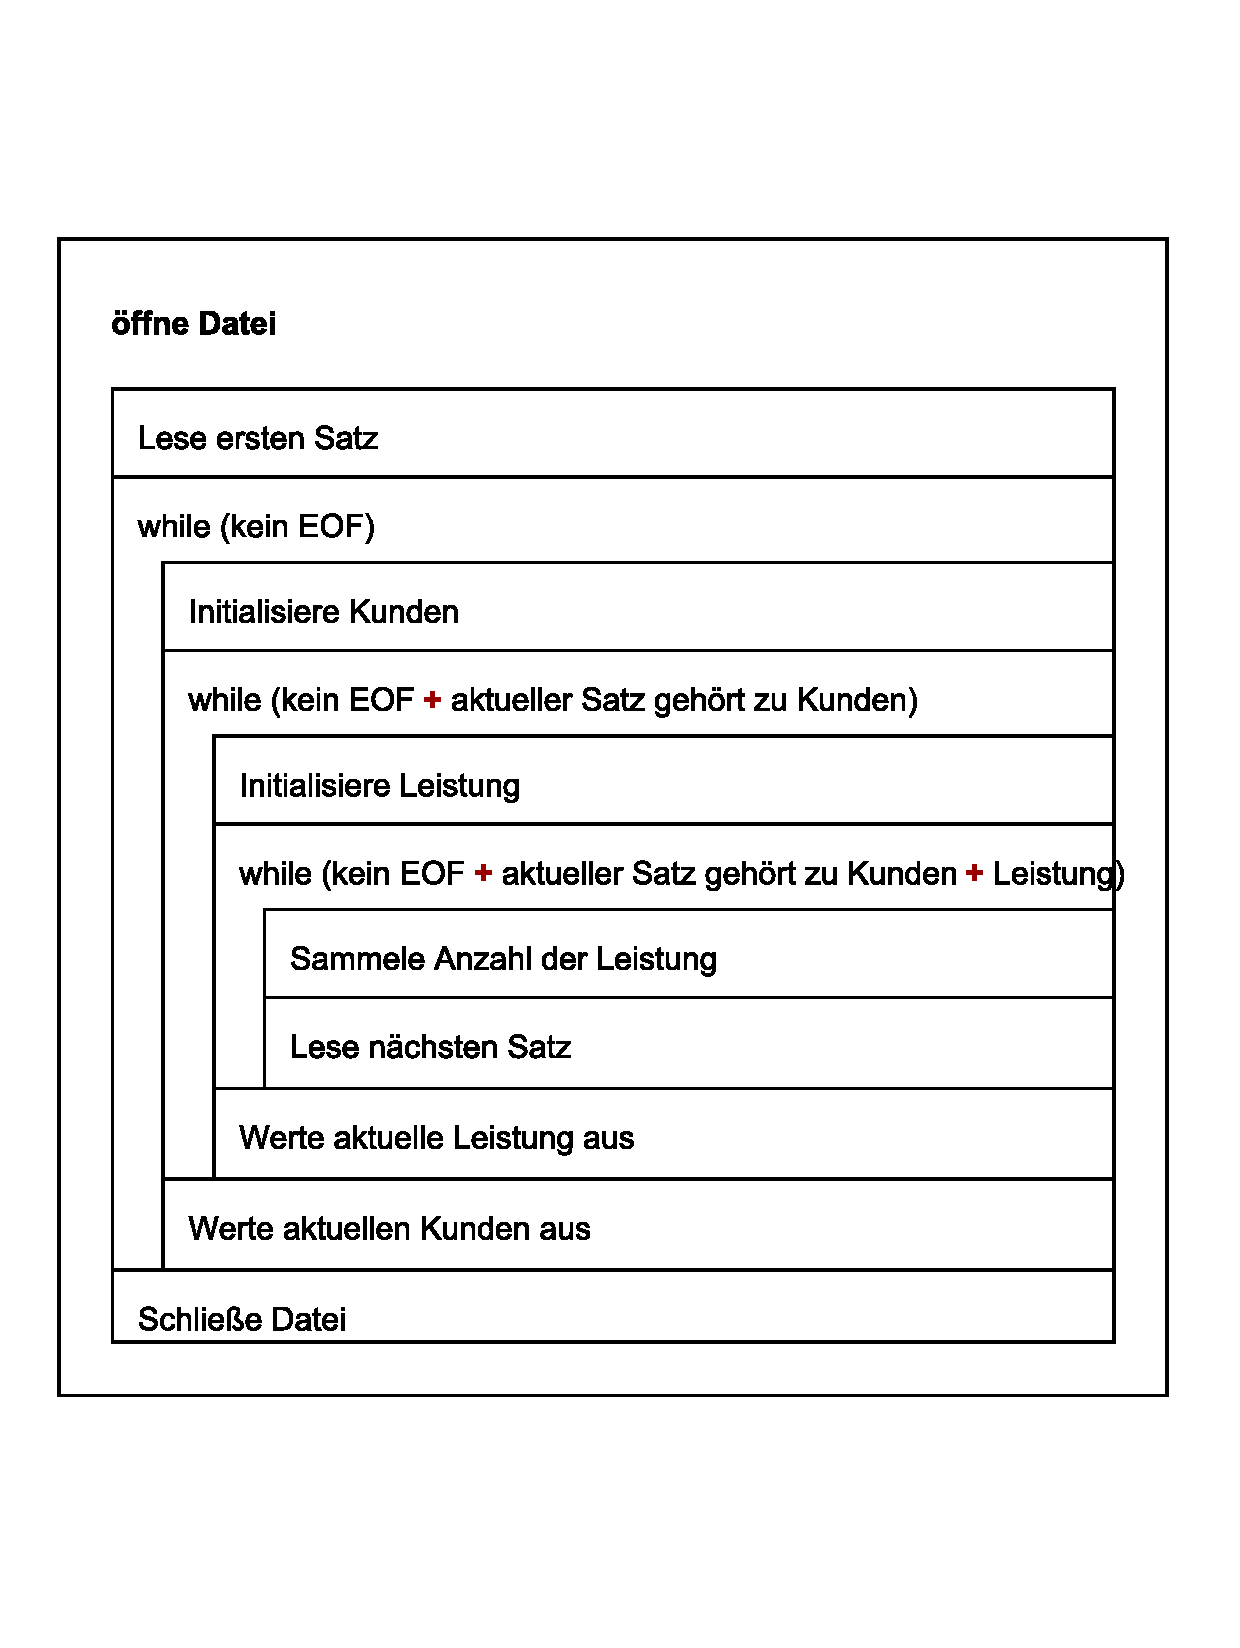
\includegraphics[width=\textwidth,height=\textheight,keepaspectratio]{images/Gruppenwechsel-NSD.pdf}
    \caption{
        Veranschaulichung des Gruppenwechsels II
    }
    \label{fig:diagramm2}
\end{figure}

\begin{figure}[!h]
    \centering
    \includegraphics[width=\textwidth,height=\textheight,keepaspectratio]{images/Erhalte_Leistungsbezeichnung-PAP.pdf}
    \caption{
        Ablauf der Ermittlung der Leistungsbezeichnugnen
    }
    \label{fig:diagramm3}
\end{figure}



\section{Entwicklungsdokumentation}\label{sec:entwicklerdokumentation}
Es wurden grundsätzlich sprechende Namen für Variablen, Abschnitte und Paragrafen gewählt. Außerdem sind \texttt{DISPLAY} Statements welche zum Debuggen genutz wurden erhalten geblieben. Mit diesen ist der Programmablauf leichter nachzuvollziehen.

Daher bedarf es nur geringer Dokumentation.
Die Funktionen der einzelnen Paragrafen sind in Tabelle~\ref{tab:prog-strukt} beschrieben.


\definecolor{fhfarbe}{HTML}{51B2AC}
\definecolor{fhfarbe2}{HTML}{4FAEAB}
\begin{table}[!htb]
    \centering
    \rowcolors{2}{black!5}{white}
    \begin{tabularx}{\textwidth}{X | X }
       \rowcolor{fhfarbe!25}
       Bezeichnung                             & Beschreibung             \\
%       \hline
       \rowcolor{fhfarbe!10}
       MAIN-PROCEDURE & Hauptablauf welcher den Gruppenwechsel delegiert \\
       PREPERATION & Spiegelt den Vorlauf zum einlesen einer Datei wieder und öffnet die Einlsese- (JOURNAL.txt) und Auslesedatei (INVOICE.txt) \\
       CUSTOMER-PREPERATION & Wertet den akutellen Einlesesatz aus und initialisiert daraus einen Kunden \\
       SERVICE-PREPERATION & Wertet den aktuellen Einlesesatz weiter aus und initialisiert daraus eine Leistung \\
       INDIVIDUAL-PROCESSING & Wertet den aktuellen Einlesesatz aus und zählt die Vorkommensanzahl einer Leistung hoch \\
       READ-NEXT-LINE & Liest, wenn möglich, die nächste Zeile des Jounrals ein \\
       SERVICE-COMPLETION & Wertet die aktuelle Leistung aus indem der Gesamtbetrag der Leistung berechnet und mit allen relevanten Leistungsdaten in die Rechnung geschrieben wird \\
       CUSTOMER-COMPLETION & Wertet den aktuellen Kunden aus indem der Gesamtbetrag des Kunden in die Rechnung geschrieben und ein Ende gekennzeichnet wird \\
       COMPLETION & schließt Einlese- und Auslesedatei \\
       
       \rowcolor{fhfarbe!10}
       GET-SERVICE-TERM & Ermittelt anhand der Leistungs-ID durch einlesen des Leistungsglossar die Leistungsbeschreibung \\
       CHECK-LINE & Überprüft, ob die aktuell aus dem Glossar eingelesene Leistungs-ID mit der zu überprüfenden Leistungs-ID übereinstimmt \\
       NEXT-LINE & Liest, wenn möglich die nächste Zeile des Glossars ein\\
       DISPLAY-JOURNAL & Debugeinheit zum ausgeben der aktuell eingelesenen Daten \\
    \end{tabularx}
    \caption{Aufgaben der einzelnen logischen Einheiten.}\label{tab:prog-strukt}
\end{table}

    \addtocontents{toc}{\protect\newpage}
    \chapter{Testdokumentation}\label{ch:testdokumentation}
Alle Testfälle können wie beschrieben in~\enquote{\nameref{sec:testen-der-beispiele}}~ausgeführt werden.
Für eine klare Struktur wurden Sie in 5 verschiedene Testgruppen eingeteilt:
\begin{enumerate}[label={\textbf{Gruppe~\arabic*:}}, ref={Gruppe~\arabic*}, leftmargin=*, noitemsep]
    \label{enm:tesgruppen}
    \item Tests, welche aus der Aufgabenstellung hervorgehen.
    \item Überprüfungen der Eingabe im T9- bzw. Normalmodus.
    \item Überprüfungen der Eingabe im Explizitmodus.
    \item Tests, welche speziell auf die Semantik im Explizitmodus eingehen.
    \item Tests, welche die Reihenfolge der Wortvorschläge überprüfen
    \item Tests, welche das Einlesen und Ausgeben von Wörterbüchern überprüfen.
    \item Tests, zum Überprüfen der beschriebenen Sonderfälle (Kapitel~\ref{subsec:sonderfaelle})
\end{enumerate}

\definecolor{fhfarbe}{HTML}{00605E}


\section{Definierte Tests}\label{sec:definierte-tests}
Die in der Aufgabenstellung definierten Tests werden im Folgenden ausführlich beschrieben.
Dabei werden die allgemeine Funktionalität des Programms getestet und Normalfälle von vielen Programmkomponenten abgedeckt.
\subsection*{Normalfälle}\label{subsec:def-normalfaelle}

\paragraph*{T1.1}
Beginnend mit einem Leeren Wörterbuch wird getestet, ob der Satz \glqq DER HUT IST EIN FES.\grqq{} gebildet werden kann.
Wörterbuch:
\begin{lstlisting}[escapechar=\%]
Moechten Sie ein externes Woerterbuch einlesen? ja (*) / nein (#)
%\textcolor{fhfarbe}{\#}%
Kein Woerterbuch geladen.
Beginnen Sie einen neuen Satz oder beenden Sie das Programm mit (0).
Bitte geben Sie ein kodiertes Wort ein:
%\textcolor{fhfarbe}{3371}%
Im Woerterbuch wurde keine passender Eintrag gefunden!
Bitte Wort im Explizit-Modus eingeben:
%\textcolor{fhfarbe}{3132731}%
DER
Wort in Ordnung? ja (*) / nein (#)
%\textcolor{fhfarbe}{*}%
Das Wort DER wurde mit Code 337 im Woerterbuch abgespeichert!
Bitte geben Sie ein kodiertes Wort ein:
%\textcolor{fhfarbe}{4881}%
Im Woerterbuch wurde keine passender Eintrag gefunden!
Bitte Wort im Explizit-Modus eingeben:
%\textcolor{fhfarbe}{4282811}%
HUT
Wort in Ordnung? ja (*) / nein (#)
%\textcolor{fhfarbe}{*}%
Das Wort HUT wurde mit Code 488 im Woerterbuch abgespeichert!
Bitte geben Sie ein kodiertes Wort ein:
%\textcolor{fhfarbe}{4781}%
Im Woerterbuch wurde keine passender Eintrag gefunden!
Bitte Wort im Explizit-Modus eingeben:
%\textcolor{fhfarbe}{4374811}%
IST
Wort in Ordnung? ja (*) / nein (#)
%\textcolor{fhfarbe}{*}%
Das Wort IST wurde mit Code 478 im Woerterbuch abgespeichert!
Bitte geben Sie ein kodiertes Wort ein:
%\textcolor{fhfarbe}{3461}%
Im Woerterbuch wurde keine passender Eintrag gefunden!
Bitte Wort im Explizit-Modus eingeben:
%\textcolor{fhfarbe}{3243621}%
EIN
Wort in Ordnung? ja (*) / nein (#)
%\textcolor{fhfarbe}{*}%
Das Wort EIN wurde mit Code 346 im Woerterbuch abgespeichert!
Bitte geben Sie ein kodiertes Wort ein:
%\textcolor{fhfarbe}{3370}%
DER
Wort in Ordnung? ja (*) / nein (#)
%\textcolor{fhfarbe}{\#}%
Bitte Wort im Explizit-Modus eingeben:
%\textcolor{fhfarbe}{3332740}%
FES
Wort in Ordnung? ja (*) / nein (#)
%\textcolor{fhfarbe}{*}%
Das Wort FES wurde mit Code 337 im Woerterbuch abgespeichert!
Eingegebener Satz:
DER HUT IST EIN FES.
Beginnen Sie einen neuen Satz oder beenden Sie das Programm mit (0).
Bitte geben Sie ein kodiertes Wort ein:
%\textcolor{fhfarbe}{0}%
Programm Ende.
\end{lstlisting}

\begin{center}
    \fbox{\begin{minipage}{15em}
              337 DER 1 \\
              346 EIN 1 \\
              337 FES 1 \\
              488 HUT 1 \\
              478 IST 1
    \end{minipage}}
    \captionof{figure}{Wörterbuch nach Test 1.1.}
    \label{fig:wbuch1}
\end{center}
\paragraph*{T1.2} Es sollen die beiden Sätze \glqq DER SATZ IST KURZ. EIN FES IST EIN HUT.\grqq{} konstruiert werden.
Dabei wird das Wörterbuch~\ref{fig:wbuch1} aus dem vorherigen Test verwendet.
\begin{lstlisting}[escapechar=\%]
Moechten Sie ein externes Woerterbuch einlesen? ja (*) / nein (#)
%\textcolor{fhfarbe}{*}%
Bitte geben sie den Dateinamen des Woerterbuchs ein.
%\textcolor{fhfarbe}{Woerterbuch-out.txt}%
Woerterbuch erfolgreich eingelesen.
Beginnen Sie einen neuen Satz oder beenden Sie das Programm mit (0).
Bitte geben Sie ein kodiertes Wort ein:
%\textcolor{fhfarbe}{3371}%
DER
Wort in Ordnung? ja (*) / nein (#)
%\textcolor{fhfarbe}{*}%
Bitte geben Sie ein kodiertes Wort ein:
%\textcolor{fhfarbe}{72891}%
Im Woerterbuch wurde keine passender Eintrag gefunden!
Bitte Wort im Explizit-Modus eingeben:
%\textcolor{fhfarbe}{742181941}%
SATZ
Wort in Ordnung? ja (*) / nein (#)
%\textcolor{fhfarbe}{*}%
Das Wort SATZ wurde mit Code 7289 im Woerterbuch abgespeichert!
Bitte geben Sie ein kodiertes Wort ein:
%\textcolor{fhfarbe}{4781}%
IST
Wort in Ordnung? ja (*) / nein (#)
%\textcolor{fhfarbe}{*}%
Bitte geben Sie ein kodiertes Wort ein:
%\textcolor{fhfarbe}{58790}%
Im Woerterbuch wurde keine passender Eintrag gefunden!
Bitte Wort im Explizit-Modus eingeben:
%\textcolor{fhfarbe}{528273940}%
KURZ
Wort in Ordnung? ja (*) / nein (#)
%\textcolor{fhfarbe}{*}%
Das Wort KURZ wurde mit Code 5879 im Woerterbuch abgespeichert!
Eingegebener Satz:
DER SATZ IST KURZ.
Beginnen Sie einen neuen Satz oder beenden Sie das Programm mit (0).
Bitte geben Sie ein kodiertes Wort ein:
%\textcolor{fhfarbe}{3461}%
EIN
Wort in Ordnung? ja (*) / nein (#)
%\textcolor{fhfarbe}{*}%
Bitte geben Sie ein kodiertes Wort ein:
%\textcolor{fhfarbe}{3371}%
DER
Wort in Ordnung? ja (*) / nein (#)
%\textcolor{fhfarbe}{\#}%
FES
Wort in Ordnung? ja (*) / nein (#)
%\textcolor{fhfarbe}{*}%
Bitte geben Sie ein kodiertes Wort ein:
%\textcolor{fhfarbe}{4781}%
IST
Wort in Ordnung? ja (*) / nein (#)
%\textcolor{fhfarbe}{*}%
Bitte geben Sie ein kodiertes Wort ein:
%\textcolor{fhfarbe}{3461}%
EIN
Wort in Ordnung? ja (*) / nein (#)
%\textcolor{fhfarbe}{*}%
Bitte geben Sie ein kodiertes Wort ein:
%\textcolor{fhfarbe}{4880}%
HUT
Wort in Ordnung? ja (*) / nein (#)
%\textcolor{fhfarbe}{*}%
Eingegebener Satz:
EIN FES IST EIN HUT.
Beginnen Sie einen neuen Satz oder beenden Sie das Programm mit (0).
Bitte geben Sie ein kodiertes Wort ein:
%\textcolor{fhfarbe}{0}%
Programm Ende.
\end{lstlisting}
\begin{center}
    \fbox{\begin{minipage}{15em}
              337 DER 2 \\
              346 EIN 3\\
              337 FES 2\\
              488 HUT 2\\
              478 IST 3\\
              5879 KURZ 1\\
              7289 SATZ 1
    \end{minipage}}
    \captionof{figure}{Wörterbuch nach Test 1.2.}
    \label{fig:wbuch2}
\end{center}


\section{Normalmodus-Tests}\label{sec:normalmodus-tests}
In den folgenden Testfällen wird geprüft, ob das Programm bei Verletzung der in Kapitel~\ref{subsec:syntaktische-fehler} syntaktischen Regeln für den normalen Modus passend reagiert.
In allen Fällen sollte ein Fehler gemeldet und eine neue Eingabe gefordert werden.

\subsection*{Fehlerfälle}\label{subsec:normalmodus-fehlerfaelle}

\paragraph*{T2.1} Leerzeichen im Wort.
\begin{lstlisting}[escapechar=\%]
Bitte geben Sie ein kodiertes Wort ein:
%\textcolor{fhfarbe}{76 3892730}%
Leerzeichen innerhalb des Wortes sind nicht erlaubt!
Bitte geben Sie ein kodiertes Wort ein:
\end{lstlisting}

\paragraph*{T2.2} Ungültiges Wortende.
\begin{lstlisting}[escapechar=\%]
Bitte geben Sie ein kodiertes Wort ein:
%\textcolor{fhfarbe}{76389273}%
Es muss genau ein Leerzeichen (1) oder Punkt (0) am Wortende stehen!
Bitte geben Sie ein kodiertes Wort ein:
\end{lstlisting}

\paragraph*{T2.3} Unerlaubte Zeichen-Eingabe.
\begin{lstlisting}[escapechar=\%]
Bitte geben Sie ein kodiertes Wort ein:
%\textcolor{fhfarbe}{76389g2a730}%
Die Eingabe darf nur Ziffern von 0-9 enthalten!
Bitte geben Sie ein kodiertes Wort ein:
\end{lstlisting}

\paragraph*{T2.4} Zeichen nach Wortende.
\begin{lstlisting}[escapechar=\%]
Bitte geben Sie ein kodiertes Wort ein:
%\textcolor{fhfarbe}{763890273}%
Nach dem Leerzeichen bzw. Punkt duerfen keine weiteren Zeichen folgen!
Bitte geben Sie ein kodiertes Wort ein:
\end{lstlisting}

\paragraph*{T2.5} Mehr als ein Wortende.
\begin{lstlisting}[escapechar=\%]
Bitte geben Sie ein kodiertes Wort ein:
%\textcolor{fhfarbe}{7638927310}%
Es muss genau ein Leerzeichen (1) oder Punkt (0) am Wortende stehen!
Bitte geben Sie ein kodiertes Wort ein:
\end{lstlisting}

\paragraph*{T2.6} Leerzeichen im Wort und ungültiges Ende.
\begin{lstlisting}[escapechar=\%]
Bitte geben Sie ein kodiertes Wort ein:
%\textcolor{fhfarbe}{76 389273}%
Leerzeichen innerhalb des Wortes sind nicht erlaubt!
Es muss genau ein Leerzeichen (1) oder Punkt (0) am Wortende stehen!
Bitte geben Sie ein kodiertes Wort ein:
\end{lstlisting}

\paragraph*{T2.7} Leerzeichen im Wort und unerlaubte Zeichen.
\begin{lstlisting}[escapechar=\%]
Bitte geben Sie ein kodiertes Wort ein:
%\textcolor{fhfarbe}{763 89g2a730}%
Die Eingabe darf nur Ziffern von 0-9 enthalten!
Leerzeichen innerhalb des Wortes sind nicht erlaubt!
Bitte geben Sie ein kodiertes Wort ein:
\end{lstlisting}

\paragraph*{T2.8} Leerzeichen im Wort und Zeichen nach Wortende.
\begin{lstlisting}[escapechar=\%]
Bitte geben Sie ein kodiertes Wort ein:
%\textcolor{fhfarbe}{7638902 73}%
Leerzeichen innerhalb des Wortes sind nicht erlaubt!
Nach dem Leerzeichen bzw. Punkt duerfen keine weiteren Zeichen folgen!
Bitte geben Sie ein kodiertes Wort ein:
\end{lstlisting}

\paragraph*{T2.9} Leerzeichen im Wort und mehrfaches Wortende.
\begin{lstlisting}[escapechar=\%]
Bitte geben Sie ein kodiertes Wort ein:
%\textcolor{fhfarbe}{76389 27310}%
Leerzeichen innerhalb des Wortes sind nicht erlaubt!
Es muss genau ein Leerzeichen (1) oder Punkt (0) am Wortende stehen!
Bitte geben Sie ein kodiertes Wort ein:
\end{lstlisting}

\paragraph*{T2.10} Unerlaubte Zeichen und fehlendes Wortende.
\begin{lstlisting}[escapechar=\%]
Bitte geben Sie ein kodiertes Wort ein:
%\textcolor{fhfarbe}{76389g2a73}%
Die Eingabe darf nur Ziffern von 0-9 enthalten!
Es muss genau ein Leerzeichen (1) oder Punkt (0) am Wortende stehen!
Bitte geben Sie ein kodiertes Wort ein:
\end{lstlisting}

\paragraph*{T2.11} Unerlaubte Zeichen und Zeichen nach Wortende.
\begin{lstlisting}[escapechar=\%]
Bitte geben Sie ein kodiertes Wort ein:
%\textcolor{fhfarbe}{76389g2a703}%
Die Eingabe darf nur Ziffern von 0-9 enthalten!
Nach dem Leerzeichen bzw. Punkt duerfen keine weiteren Zeichen folgen!
Bitte geben Sie ein kodiertes Wort ein:
\end{lstlisting}

\paragraph*{T2.12} Unerlaubte Zeichen und mehrfaches Wortende.
\begin{lstlisting}[escapechar=\%]
Bitte geben Sie ein kodiertes Wort ein:
%\textcolor{fhfarbe}{76389g2a7310}%
Die Eingabe darf nur Ziffern von 0-9 enthalten!
Es muss genau ein Leerzeichen (1) oder Punkt (0) am Wortende stehen!
Bitte geben Sie ein kodiertes Wort ein:
\end{lstlisting}

\paragraph*{T2.13} Mehrfaches Wortende und Zeichen nach Wortende.
\begin{lstlisting}[escapechar=\%]
Bitte geben Sie ein kodiertes Wort ein:
%\textcolor{fhfarbe}{76389027310}%
Es muss genau ein Leerzeichen (1) oder Punkt (0) am Wortende stehen!
Bitte geben Sie ein kodiertes Wort ein:
\end{lstlisting}

\paragraph*{T2.14} Leerzeichen im Wort und unerlaubte Zeichen und fehlendes Wortende.
\begin{lstlisting}[escapechar=\%]
Bitte geben Sie ein kodiertes Wort ein:
%\textcolor{fhfarbe}{76389g2 a73}%
Die Eingabe darf nur Ziffern von 0-9 enthalten!
Leerzeichen innerhalb des Wortes sind nicht erlaubt!
Es muss genau ein Leerzeichen (1) oder Punkt (0) am Wortende stehen!
Bitte geben Sie ein kodiertes Wort ein:
\end{lstlisting}

\paragraph*{T2.15} Alle vorherigen Fehler nacheinander und anschliessend korrekte Eingabe.
\begin{lstlisting}[escapechar=\%]
Bitte geben Sie ein kodiertes Wort ein:
%\textcolor{fhfarbe}{76 3892730}%
Leerzeichen innerhalb des Wortes sind nicht erlaubt!
Bitte geben Sie ein kodiertes Wort ein:
%\textcolor{fhfarbe}{76389273}%
Es muss genau ein Leerzeichen (1) oder Punkt (0) am Wortende stehen!
Bitte geben Sie ein kodiertes Wort ein:
%\textcolor{fhfarbe}{76389g2a730}%
Die Eingabe darf nur Ziffern von 0-9 enthalten!
Bitte geben Sie ein kodiertes Wort ein:
%\textcolor{fhfarbe}{763890273}%
Nach dem Leerzeichen bzw. Punkt duerfen keine weiteren Zeichen folgen!
Bitte geben Sie ein kodiertes Wort ein:
%\textcolor{fhfarbe}{7638927310}%
Es muss genau ein Leerzeichen (1) oder Punkt (0) am Wortende stehen!
Bitte geben Sie ein kodiertes Wort ein:
%\textcolor{fhfarbe}{76 389273}%
Leerzeichen innerhalb des Wortes sind nicht erlaubt!
Es muss genau ein Leerzeichen (1) oder Punkt (0) am Wortende stehen!
Bitte geben Sie ein kodiertes Wort ein:
%\textcolor{fhfarbe}{763 89g2a730}%
Die Eingabe darf nur Ziffern von 0-9 enthalten!
Leerzeichen innerhalb des Wortes sind nicht erlaubt!
Bitte geben Sie ein kodiertes Wort ein:
%\textcolor{fhfarbe}{7638902 73}%
Leerzeichen innerhalb des Wortes sind nicht erlaubt!
Nach dem Leerzeichen bzw. Punkt duerfen keine weiteren Zeichen folgen!
Bitte geben Sie ein kodiertes Wort ein:
%\textcolor{fhfarbe}{76389 27310}%
Leerzeichen innerhalb des Wortes sind nicht erlaubt!
Es muss genau ein Leerzeichen (1) oder Punkt (0) am Wortende stehen!
Bitte geben Sie ein kodiertes Wort ein:
%\textcolor{fhfarbe}{76389g2a73}%
Die Eingabe darf nur Ziffern von 0-9 enthalten!
Es muss genau ein Leerzeichen (1) oder Punkt (0) am Wortende stehen!
Bitte geben Sie ein kodiertes Wort ein:
%\textcolor{fhfarbe}{76389g2a703}%
Die Eingabe darf nur Ziffern von 0-9 enthalten!
Nach dem Leerzeichen bzw. Punkt duerfen keine weiteren Zeichen folgen!
Bitte geben Sie ein kodiertes Wort ein:
%\textcolor{fhfarbe}{76389g2a7310}%
Die Eingabe darf nur Ziffern von 0-9 enthalten!
Es muss genau ein Leerzeichen (1) oder Punkt (0) am Wortende stehen!
Bitte geben Sie ein kodiertes Wort ein:
%\textcolor{fhfarbe}{76389027310}%
Es muss genau ein Leerzeichen (1) oder Punkt (0) am Wortende stehen!
Bitte geben Sie ein kodiertes Wort ein:
%\textcolor{fhfarbe}{76389g2 a73}%
Die Eingabe darf nur Ziffern von 0-9 enthalten!
Leerzeichen innerhalb des Wortes sind nicht erlaubt!
Es muss genau ein Leerzeichen (1) oder Punkt (0) am Wortende stehen!
Bitte geben Sie ein kodiertes Wort ein:
%\textcolor{fhfarbe}{763892730}%
Im Woerterbuch wurde keine passender Eintrag gefunden!
Bitte Wort im Explizit-Modus eingeben:
%\textcolor{fhfarbe}{74633381912173320}%
 SOFTWARE
Wort in Ordnung? ja (*) / nein (#)
%\textcolor{fhfarbe}{*}%
Das Wort SOFTWARE wurde mit Code 76389273 im Woerterbuch abgespeichert!
Eingegebener Satz:
 SOFTWARE.
\end{lstlisting}

\subsection*{Grenzfälle}\label{subsec:normalmodus-grenzfaelle}

\paragraph*{T2.16} Zu kurze Eingabe.
\begin{lstlisting}[escapechar=\%]
Bitte geben Sie ein kodiertes Wort ein:
%\textcolor{fhfarbe}{1}%
Das Wort sollte mindestens einen Buchstaben enthalten!
Bitte geben Sie ein kodiertes Wort ein:
\end{lstlisting}

\paragraph*{T2.17} Eingabe ist zu lang.
\begin{lstlisting}[escapechar=\%]
Bitte geben Sie ein kodiertes Wort ein:
%\textcolor{fhfarbe}{763892732323332240}%
Wort zu lang! Es sind hoechstens 16 Ziffern erlaubt (15 Buchstaben und 1 Wort-Ende)!
Es muss genau ein Leerzeichen (1) oder Punkt (0) am Wortende stehen!
Bitte geben Sie ein kodiertes Wort ein:
\end{lstlisting}


\section{Explizitmodus-Eingabe-Tests}\label{sec:explizitmodus-tests}

In den folgenden Testfällen wird geprüft, ob das Programm bei Verletzung der in Kapitel~\ref{subsec:syntaktische-fehler} syntaktischen Regeln für den Explizitmodus, passend reagiert.
In allen Fällen sollte ein Fehler gemeldet und eine neue Eingabe gefordert werden.

\subsection*{Fehlerfälle}\label{subsec:explizit-fehlerfaelle}

\paragraph*{T3.1} Unerlaubte Zeichen.
\begin{lstlisting}[escapechar=\%]
Bitte Wort im Explizit-Modus eingeben:
%\textcolor{fhfarbe}{3343g7423420}%
Die Eingabe darf nur Ziffern von 0-9 enthalten!
Bitte Wort im Explizit-Modus eingeben:
\end{lstlisting}

\paragraph*{T3.2} Leerzeichen im Wort.
\begin{lstlisting}[escapechar=\%]
Bitte Wort im Explizit-Modus eingeben:
%\textcolor{fhfarbe}{3343 7423420}%
Leerzeichen innerhalb des Wortes sind nicht erlaubt!
Bitte Wort im Explizit-Modus eingeben:
\end{lstlisting}

\paragraph*{T3.3} Gerade Anzahl von Ziffern.
\begin{lstlisting}[escapechar=\%]
Bitte Wort im Explizit-Modus eingeben:
%\textcolor{fhfarbe}{334327423420}%
Es wurde eine gerade Zahl von Ziffern eingeben. Im Explizitmodus werden buchstaben als Paare kodiert, das Abschliessende Symbol (Punkt (0) oder Leerzeichen (1)) wird aber nur einmal eingegeben!
Bitte Wort im Explizit-Modus eingeben:
\end{lstlisting}

\paragraph*{T3.4} Ungültiges Wortende.
\begin{lstlisting}[escapechar=\%]
Bitte Wort im Explizit-Modus eingeben:
%\textcolor{fhfarbe}{33437423423}%
Das Wort wurde mit keinem Gueltigen Zeichen (0 oder 1) abgeschlossen!
Bitte Wort im Explizit-Modus eingeben:
\end{lstlisting}

\paragraph*{T3.5} Unerlaubte Zeichen und Leerzeichen im Wort.
\begin{lstlisting}[escapechar=\%]
Bitte Wort im Explizit-Modus eingeben:
%\textcolor{fhfarbe}{3343g74 23420}%
Die Eingabe darf nur Ziffern von 0-9 enthalten!
Leerzeichen innerhalb des Wortes sind nicht erlaubt!
Bitte Wort im Explizit-Modus eingeben:
\end{lstlisting}

\paragraph*{T3.6} Unerlaubte Zeichen und gerade Anzahl von Ziffern.
\begin{lstlisting}[escapechar=\%]
Bitte Wort im Explizit-Modus eingeben:
%\textcolor{fhfarbe}{3343g743420}%
Die Eingabe darf nur Ziffern von 0-9 enthalten!
Es wurde eine gerade Zahl von Ziffern eingeben. Im Explizitmodus werden buchstaben als Paare kodiert, das Abschliessende Symbol (Punkt (0) oder Leerzeichen (1)) wird aber nur einmal eingegeben!
Bitte Wort im Explizit-Modus eingeben:
\end{lstlisting}

\paragraph*{T3.7} Unerlaubte Zeichen und ungueltiges Wortende.
\begin{lstlisting}[escapechar=\%]
Bitte Wort im Explizit-Modus eingeben:
%\textcolor{fhfarbe}{3343g7423424}%
Die Eingabe darf nur Ziffern von 0-9 enthalten!
Das Wort wurde mit keinem Gueltigen Zeichen (0 oder 1) abgeschlossen!
Bitte Wort im Explizit-Modus eingeben:
\end{lstlisting}

\paragraph*{T3.8} Leerzeichen im Wort und gerade Anzahl von Ziffern.
\begin{lstlisting}[escapechar=\%]
Bitte Wort im Explizit-Modus eingeben:
%\textcolor{fhfarbe}{33432 7423420}%
Leerzeichen innerhalb des Wortes sind nicht erlaubt!
Es wurde eine gerade Zahl von Ziffern eingeben. Im Explizitmodus werden buchstaben als Paare kodiert, das Abschliessende Symbol (Punkt (0) oder Leerzeichen (1)) wird aber nur einmal eingegeben!
Bitte Wort im Explizit-Modus eingeben:
\end{lstlisting}

\paragraph*{T3.9} Leerzeichen im Wort und ungueltiges Wortende.
\begin{lstlisting}[escapechar=\%]
Bitte Wort im Explizit-Modus eingeben:
%\textcolor{fhfarbe}{334374 23423}%
Leerzeichen innerhalb des Wortes sind nicht erlaubt!
Das Wort wurde mit keinem Gueltigen Zeichen (0 oder 1) abgeschlossen!
Bitte Wort im Explizit-Modus eingeben:
\end{lstlisting}

\paragraph*{T3.10} Gerade Anzahl von Ziffern und ungültiges Wortende.
\begin{lstlisting}[escapechar=\%]
Bitte Wort im Explizit-Modus eingeben:
%\textcolor{fhfarbe}{3343742342}%
Es wurde eine gerade Zahl von Ziffern eingeben. Im Explizitmodus werden buchstaben als Paare kodiert, das Abschliessende Symbol (Punkt (0) oder Leerzeichen (1)) wird aber nur einmal eingegeben!
Das Wort wurde mit keinem Gueltigen Zeichen (0 oder 1) abgeschlossen!
Bitte Wort im Explizit-Modus eingeben:
\end{lstlisting}

\paragraph*{T3.11} Unerlaubte Zeichen und Leerzeichen im Wort und gerade Anzahl von Ziffern.
\begin{lstlisting}[escapechar=\%]
Bitte Wort im Explizit-Modus eingeben:
%\textcolor{fhfarbe}{3343g74 234230}%
Die Eingabe darf nur Ziffern von 0-9 enthalten!
Leerzeichen innerhalb des Wortes sind nicht erlaubt!
Es wurde eine gerade Zahl von Ziffern eingeben. Im Explizitmodus werden buchstaben als Paare kodiert, das Abschliessende Symbol (Punkt (0) oder Leerzeichen (1)) wird aber nur einmal eingegeben!
Bitte Wort im Explizit-Modus eingeben:
\end{lstlisting}

\paragraph*{T3.12} Unerlaubte Zeichen und Leerzeichen im Wort und ungültiges Wortende.
\begin{lstlisting}[escapechar=\%]
Bitte Wort im Explizit-Modus eingeben:
%\textcolor{fhfarbe}{3343g74 23423}%
Die Eingabe darf nur Ziffern von 0-9 enthalten!
Leerzeichen innerhalb des Wortes sind nicht erlaubt!
Das Wort wurde mit keinem Gueltigen Zeichen (0 oder 1) abgeschlossen!
Bitte Wort im Explizit-Modus eingeben:
\end{lstlisting}

\paragraph*{T3.13} Gerade Anzahl von Ziffern und Leerzeichen im Wort und ungültiges Wortende.
\begin{lstlisting}[escapechar=\%]
Bitte Wort im Explizit-Modus eingeben:
%\textcolor{fhfarbe}{334374 2342}%
Leerzeichen innerhalb des Wortes sind nicht erlaubt!
Es wurde eine gerade Zahl von Ziffern eingeben. Im Explizitmodus werden buchstaben als Paare kodiert, das Abschliessende Symbol (Punkt (0) oder Leerzeichen (1)) wird aber nur einmal eingegeben!
Das Wort wurde mit keinem Gueltigen Zeichen (0 oder 1) abgeschlossen!
Bitte Wort im Explizit-Modus eingeben:
\end{lstlisting}

\paragraph*{T3.14} Gerade Anzahl von Ziffern und Leerzeichen im Wort und ungültiges Wortende und ungültige Zeichen.
\begin{lstlisting}[escapechar=\%]
Bitte Wort im Explizit-Modus eingeben:
%\textcolor{fhfarbe}{3343z74 2342}%
Die Eingabe darf nur Ziffern von 0-9 enthalten!
Leerzeichen innerhalb des Wortes sind nicht erlaubt!
Es wurde eine gerade Zahl von Ziffern eingeben. Im Explizitmodus werden buchstaben als Paare kodiert, das Abschliessende Symbol (Punkt (0) oder Leerzeichen (1)) wird aber nur einmal eingegeben!
Das Wort wurde mit keinem Gueltigen Zeichen (0 oder 1) abgeschlossen!
Bitte Wort im Explizit-Modus eingeben:
\end{lstlisting}

\paragraph*{T3.15} Alle oben stehenden Fehler hintereinander.
\begin{lstlisting}[escapechar=\%]
Bitte Wort im Explizit-Modus eingeben:
%\textcolor{fhfarbe}{3343g7423420}%
Die Eingabe darf nur Ziffern von 0-9 enthalten!
Bitte Wort im Explizit-Modus eingeben:
%\textcolor{fhfarbe}{3343 7423420}%
Leerzeichen innerhalb des Wortes sind nicht erlaubt!
Bitte Wort im Explizit-Modus eingeben:
%\textcolor{fhfarbe}{334327423420}%
Es wurde eine gerade Zahl von Ziffern eingeben. Im Explizitmodus werden buchstaben als Paare kodiert, das Abschliessende Symbol (Punkt (0) oder Leerzeichen (1)) wird aber nur einmal eingegeben!
Bitte Wort im Explizit-Modus eingeben:
%\textcolor{fhfarbe}{33437423423}%
Das Wort wurde mit keinem Gueltigen Zeichen (0 oder 1) abgeschlossen!
Bitte Wort im Explizit-Modus eingeben:
%\textcolor{fhfarbe}{3343g74 23420}%
Die Eingabe darf nur Ziffern von 0-9 enthalten!
Leerzeichen innerhalb des Wortes sind nicht erlaubt!
Bitte Wort im Explizit-Modus eingeben:
%\textcolor{fhfarbe}{3343g743420}%
Die Eingabe darf nur Ziffern von 0-9 enthalten!
Es wurde eine gerade Zahl von Ziffern eingeben. Im Explizitmodus werden buchstaben als Paare kodiert, das Abschliessende Symbol (Punkt (0) oder Leerzeichen (1)) wird aber nur einmal eingegeben!
Bitte Wort im Explizit-Modus eingeben:
%\textcolor{fhfarbe}{3343g7423424}%
Die Eingabe darf nur Ziffern von 0-9 enthalten!
Das Wort wurde mit keinem Gueltigen Zeichen (0 oder 1) abgeschlossen!
Bitte Wort im Explizit-Modus eingeben:
%\textcolor{fhfarbe}{33432 7423420}%
Leerzeichen innerhalb des Wortes sind nicht erlaubt!
Es wurde eine gerade Zahl von Ziffern eingeben. Im Explizitmodus werden buchstaben als Paare kodiert, das Abschliessende Symbol (Punkt (0) oder Leerzeichen (1)) wird aber nur einmal eingegeben!
Bitte Wort im Explizit-Modus eingeben:
%\textcolor{fhfarbe}{334374 23423}%
Leerzeichen innerhalb des Wortes sind nicht erlaubt!
Das Wort wurde mit keinem Gueltigen Zeichen (0 oder 1) abgeschlossen!
Bitte Wort im Explizit-Modus eingeben:
%\textcolor{fhfarbe}{3343742342}%
Es wurde eine gerade Zahl von Ziffern eingeben. Im Explizitmodus werden buchstaben als Paare kodiert, das Abschliessende Symbol (Punkt (0) oder Leerzeichen (1)) wird aber nur einmal eingegeben!
Das Wort wurde mit keinem Gueltigen Zeichen (0 oder 1) abgeschlossen!
Bitte Wort im Explizit-Modus eingeben:
%\textcolor{fhfarbe}{3343g74 234230}%
Die Eingabe darf nur Ziffern von 0-9 enthalten!
Leerzeichen innerhalb des Wortes sind nicht erlaubt!
Es wurde eine gerade Zahl von Ziffern eingeben. Im Explizitmodus werden buchstaben als Paare kodiert, das Abschliessende Symbol (Punkt (0) oder Leerzeichen (1)) wird aber nur einmal eingegeben!
Bitte Wort im Explizit-Modus eingeben:
%\textcolor{fhfarbe}{3343g74 23423}%
Die Eingabe darf nur Ziffern von 0-9 enthalten!
Leerzeichen innerhalb des Wortes sind nicht erlaubt!
Das Wort wurde mit keinem Gueltigen Zeichen (0 oder 1) abgeschlossen!
Bitte Wort im Explizit-Modus eingeben:
%\textcolor{fhfarbe}{334374 2342}%
Leerzeichen innerhalb des Wortes sind nicht erlaubt!
Es wurde eine gerade Zahl von Ziffern eingeben. Im Explizitmodus werden buchstaben als Paare kodiert, das Abschliessende Symbol (Punkt (0) oder Leerzeichen (1)) wird aber nur einmal eingegeben!
Das Wort wurde mit keinem Gueltigen Zeichen (0 oder 1) abgeschlossen!
Bitte Wort im Explizit-Modus eingeben:
%\textcolor{fhfarbe}{3343z74 2342}%
Die Eingabe darf nur Ziffern von 0-9 enthalten!
Leerzeichen innerhalb des Wortes sind nicht erlaubt!
Es wurde eine gerade Zahl von Ziffern eingeben. Im Explizitmodus werden buchstaben als Paare kodiert, das Abschliessende Symbol (Punkt (0) oder Leerzeichen (1)) wird aber nur einmal eingegeben!
Das Wort wurde mit keinem Gueltigen Zeichen (0 oder 1) abgeschlossen!
Bitte Wort im Explizit-Modus eingeben:
%\textcolor{fhfarbe}{33437423420}%
FISCH
Wort in Ordnung? ja (*) / nein (#)
%\textcolor{fhfarbe}{*}%
Das Wort FISCH wurde mit Code 34724 im Woerterbuch abgespeichert!
Eingegebener Satz:
FISCH.
\end{lstlisting}

\subsection*{Grenzfälle}\label{subsec:explizit-grenzfaelle}

\paragraph*{T3.16} Grenzfall: Zu kurze Eingabe.
\begin{lstlisting}[escapechar=\%]
Bitte Wort im Explizit-Modus eingeben:
%\textcolor{fhfarbe}{1}%
Das Wort sollte mindestens einen Buchstaben enthalten!
Bitte Wort im Explizit-Modus eingeben:
\end{lstlisting}

\paragraph*{T3.17} Grenzfall: Eingabe ist zu lang.
\begin{lstlisting}[escapechar=\%]
Bitte Wort im Explizit-Modus eingeben:
%\textcolor{fhfarbe}{334374234222222222222222222233333333330}%
Wort zu lang! Es sind hoechstens 31 Ziffern erlaubt (15 Buchstabenpaare und 1 Wort-Ende)!
Es wurde eine gerade Zahl von Ziffern eingeben. Im Explizitmodus werden buchstaben als Paare kodiert, das Abschliessende Symbol (Punkt (0) oder Leerzeichen (1)) wird aber nur einmal eingegeben!
Das Wort wurde mit keinem Gueltigen Zeichen (0 oder 1) abgeschlossen!
Bitte Wort im Explizit-Modus eingeben:
\end{lstlisting}


\section{Semantik Explizitmodus-Tests}\label{sec:semantik-explizitmodus-tests}
In den folgenden Tests werden Explizit-Eingaben geprüft, die den syntaktischen Vorgaben genügen, aber nicht dem strukturellen Aufbau der Handytastatur entsprechen.

\subsection*{Fehlerfälle}\label{subsec:sematik-fehler}

\paragraph*{T4.1} Zugriff auf nicht existierenden Buchstaben 64.
\begin{lstlisting}[escapechar=\%]
Bitte Wort im Explizit-Modus eingeben:
%\textcolor{fhfarbe}{64218142320}%
64 ist kein gueltiger Buchstabe!
Bitte Wort im Explizit-Modus eingeben:
\end{lstlisting}

\paragraph*{T4.2} Index 65 außerhalb der maximalen Tastenlänge.
\begin{lstlisting}[escapechar=\%]
Bitte Wort im Explizit-Modus eingeben:
%\textcolor{fhfarbe}{65218142320}%
Buchstabenindex 5 des 01-ten Buchstaben zu hoch! Tasten haben maximal 4 Eintraege!
Bitte Wort im Explizit-Modus eingeben:
\end{lstlisting}

\paragraph*{T4.3} Mehrere ungültige Buchstaben.
\begin{lstlisting}[escapechar=\%]
Bitte Wort im Explizit-Modus eingeben:
%\textcolor{fhfarbe}{64248142320}%
64 ist kein gueltiger Buchstabe!
24 ist kein gueltiger Buchstabe!
Bitte Wort im Explizit-Modus eingeben:
\end{lstlisting}

\paragraph*{T4.4} Ungültiger Buchstabe und Index größer 4.
\begin{lstlisting}[escapechar=\%]
Bitte Wort im Explizit-Modus eingeben:
%\textcolor{fhfarbe}{65118142320}%
Buchstabenindex 5 des 01-ten Buchstaben zu hoch! Tasten haben maximal 4 Eintraege!
11 ist kein gueltiger Buchstabe!
Bitte Wort im Explizit-Modus eingeben:
\end{lstlisting}

\paragraph*{T4.5} Mehrere Indizes größer als 4.
\begin{lstlisting}[escapechar=\%]
Bitte Wort im Explizit-Modus eingeben:
%\textcolor{fhfarbe}{65218142390}%
Buchstabenindex 5 des 01-ten Buchstaben zu hoch! Tasten haben maximal 4 Eintraege!
Buchstabenindex 9 des 05-ten Buchstaben zu hoch! Tasten haben maximal 4 Eintraege!
Bitte Wort im Explizit-Modus eingeben:
\end{lstlisting}

\subsection*{Grenzfälle}\label{subsec:semantik-grenz}
\paragraph*{T4.6} Wort wird nicht dem Wörterbuch hinzugefügt, da es bereits voll ist. Es wird trotzdem dem Satz angehängt.
\begin{lstlisting}[escapechar=\%]
Bitte Wort im Explizit-Modus eingeben:
%\textcolor{fhfarbe}{61218142320}%
MATHE
Wort in Ordnung? ja (*) / nein (#)
%\textcolor{fhfarbe}{*}%
Das Wort konnte nicht abgespeichert werden, weil das Woerterbuch voll ist!
Eingegebener Satz:
MATHE.
\end{lstlisting}


\section{Wortvorschläge-Tests}\label{sec:wortvorschläge-tests}
\subsection*{Normalfälle}\label{subsec:vorschlag-normalfaelle}
Wörter, die einem eingegebenen T9-Code entsprechen, sollen in der Reihenfolge ihrer Häufigkeit ausgegeben werden.
\paragraph*{T5.1} Ausgabe der Wörter in richtiger Reihenfolge.
Das Wörterbuch enthält mehrere Wörter zu einem T9-Code (Zur Übersicht wurden Wörter gewählt, die nicht zum T9-Code passen):
\begin{center}
    \fbox{\begin{minipage}{15em}
              2345 DREI 3 \\
              2345 ZWEI 9 \\
              2345 VIER 2 \\
              2345 FUENF 1 \\
              2345 EINS 13
    \end{minipage}}
\end{center}
\begin{lstlisting}[escapechar=\%]
Moechten Sie ein externes Woerterbuch einlesen? ja (*) / nein (#)
%\textcolor{fhfarbe}{*}%
Bitte geben sie den Dateinamen des Woerterbuchs ein.
%\textcolor{fhfarbe}{TestWBs/WBuch-Reihenfolge.txt}%
Woerterbuch erfolgreich eingelesen.
Beginnen Sie einen neuen Satz oder beenden Sie das Programm mit (0).
Bitte geben Sie ein kodiertes Wort ein:
%\textcolor{fhfarbe}{23450}%
EINS
Wort in Ordnung? ja (*) / nein (#)
%\textcolor{fhfarbe}{\#}%
ZWEI
Wort in Ordnung? ja (*) / nein (#)
%\textcolor{fhfarbe}{\#}%
DREI
Wort in Ordnung? ja (*) / nein (#)
%\textcolor{fhfarbe}{\#}%
VIER
Wort in Ordnung? ja (*) / nein (#)
%\textcolor{fhfarbe}{\#}%
FUENF
Wort in Ordnung? ja (*) / nein (#)
%\textcolor{fhfarbe}{*}%
Eingegebener Satz:
FUENF.
\end{lstlisting}


\section{Wörterbücher-Tests}\label{sec:wörterbücher-tests}

\subsection*{Normalfälle}\label{subsec:wbuch-normalfaelle}
\paragraph*{T6.1} 6.1: Einlesen eines existierenden Wörterbuchs funktioniert fehlerfrei
\begin{lstlisting}[escapechar=\%]
Moechten Sie ein externes Woerterbuch einlesen? ja (*) / nein (#)
%\textcolor{fhfarbe}{*}%
Bitte geben Sie den Dateinamen des Woerterbuchs ein.
%\textcolor{fhfarbe}{TestWBs/WBuch-correct.txt}%
Woerterbuch erfolgreich eingelesen.
\end{lstlisting}

\paragraph*{T6.1} 6.1.1: Alle Einträge des Wörterbuchs sind verfügbar:
\begin{lstlisting}[escapechar=\%]
Moechten Sie ein externes Woerterbuch einlesen? ja (*) / nein (#)
%\textcolor{fhfarbe}{*}%
Bitte geben Sie den Dateinamen des Woerterbuchs ein.
%\textcolor{fhfarbe}{TestWBs/WBuch-correct.txt}%
Woerterbuch erfolgreich eingelesen.
Beginnen Sie einen neuen Satz oder beenden Sie das Programm mit (0).
Bitte geben Sie ein kodiertes Wort ein:
%\textcolor{fhfarbe}{763892731}%
SOFTWARE
Wort in Ordnung? ja (*) / nein (#)
%\textcolor{fhfarbe}{*}%
Bitte geben Sie ein kodiertes Wort ein:
%\textcolor{fhfarbe}{96781}%
WORT
Wort in Ordnung? ja (*) / nein (#)
%\textcolor{fhfarbe}{*}%
Bitte geben Sie ein kodiertes Wort ein:
%\textcolor{fhfarbe}{3371}%
DER
Wort in Ordnung? ja (*) / nein (#)
%\textcolor{fhfarbe}{*}%
Bitte geben Sie ein kodiertes Wort ein:
%\textcolor{fhfarbe}{3370}%
DER
Wort in Ordnung? ja (*) / nein (#)
%\textcolor{fhfarbe}{\#}%
FES
Wort in Ordnung? ja (*) / nein (#)
%\textcolor{fhfarbe}{*}%
Eingegebener Satz:
SOFTWARE WORT DER FES.
\end{lstlisting}

\subsection*{Fehlerfälle}\label{subsec:wbuch-fehlerfaelle}
\paragraph*{T6.2} Einlesen eines korrupten Wörterbuchs erzeugt Fehlermeldung.
\begin{lstlisting}[escapechar=\%]
Moechten Sie ein externes Woerterbuch einlesen? ja (*) / nein (#)
%\textcolor{fhfarbe}{*}%
Bitte geben Sie den Dateinamen des Woerterbuchs ein.
%\textcolor{fhfarbe}{TestWBs/WBuch-incorrect.txt}%
Der 1-te Satz der Datei liegt nicht im richtigen Format vor!
Wenn mit einem beschaedigten Woerterbuch gearbeitet wird, kann es zur Laufzeit zu Fehlern kommen! Beheben Sie die Syntaxfehler, lesen Sie ein anderes Woerterbuch ein oder fahren Sie fort ohne Woerterbuch.
\end{lstlisting}

\paragraph*{T6.3} Einlesen eines nicht existierenden Wörterbuchs erzeugt Fehlermeldung.
\begin{lstlisting}[escapechar=\%]
Moechten Sie ein externes Woerterbuch einlesen? ja (*) / nein (#)
%\textcolor{fhfarbe}{*}%
Bitte geben Sie den Dateinamen des Woerterbuchs ein.
%\textcolor{fhfarbe}{IDoNotExist.txt}%
Kein Woerterbuch geladen.
\end{lstlisting}

\paragraph*{T6.4} Einlesen eines leeren Wörterbuchs erzeugt Fehlermeldung.
\begin{lstlisting}[escapechar=\%]
Moechten Sie ein externes Woerterbuch einlesen? ja (*) / nein (#)
%\textcolor{fhfarbe}{*}%
Bitte geben Sie den Dateinamen des Woerterbuchs ein.
%\textcolor{fhfarbe}{TestWBs/WBuch-empty.txt}%
Woerterbuch ist leer.
Woerterbuch erfolgreich eingelesen.
\end{lstlisting}


\subsection*{Sonderfälle}\label{subsec:wbuch-sonderfaelle}
\paragraph*{T6.5} Nach Programmende enthält Wörterbuch sowohl eingelesene als auch neue Einträge.
\begin{lstlisting}[escapechar=\%]
Moechten Sie ein externes Woerterbuch einlesen? ja (*) / nein (#)
%\textcolor{fhfarbe}{*}%
Bitte geben Sie den Dateinamen des Woerterbuchs ein.
%\textcolor{fhfarbe}{TestWBs/WBuch-correct.txt}%
Woerterbuch erfolgreich eingelesen.
Beginnen Sie einen neuen Satz oder beenden Sie das Programm mit (0).
Bitte geben Sie ein kodiertes Wort ein:
%\textcolor{fhfarbe}{2581}%
ALT
Wort in Ordnung? ja (*) / nein (#)
%\textcolor{fhfarbe}{*}%
Bitte geben Sie ein kodiertes Wort ein:
%\textcolor{fhfarbe}{4241}%
Im Woerterbuch wurde kein passender Eintrag gefunden!
Bitte Wort im Explizit-Modus eingeben:
%\textcolor{fhfarbe}{4323421}%
ICH
Wort in Ordnung? ja (*) / nein (#)
%\textcolor{fhfarbe}{*}%
Das Wort ICH wurde mit Code 424 im Woerterbuch abgespeichert!
Bitte geben Sie ein kodiertes Wort ein:
%\textcolor{fhfarbe}{2461}%
Im Woerterbuch wurde kein passender Eintrag gefunden!
Bitte Wort im Explizit-Modus eingeben:
%\textcolor{fhfarbe}{2243621}%
BIN
Wort in Ordnung? ja (*) / nein (#)
%\textcolor{fhfarbe}{*}%
Das Wort BIN wurde mit Code 246 im Woerterbuch abgespeichert!
Bitte geben Sie ein kodiertes Wort ein:
%\textcolor{fhfarbe}{6380}%
Im Woerterbuch wurde kein passender Eintrag gefunden!
Bitte Wort im Explizit-Modus eingeben:
%\textcolor{fhfarbe}{6232820}%
NEU
Wort in Ordnung? ja (*) / nein (#)
%\textcolor{fhfarbe}{*}%
Das Wort NEU wurde mit Code 638 im Woerterbuch abgespeichert!
Eingegebener Satz:
ALT ICH BIN NEU.
\end{lstlisting}

\begin{center}
    \fbox{\begin{minipage}{15em}
              258 ALT 1 \\
              246 BIN 1 \\
              424 ICH 1 \\
              638 NEU 1
    \end{minipage}}
    \captionof{figure}{Wörterbuch nach Test 6.5}
    \label{fig:wbuch4}
\end{center}
\subsection*{Grenzfall}\label{subsec:wbuch-grenzfaelle}
\paragraph*{T6.2} Grenzfall: Textdatei hat mehr Einträge als interne Datenstruktur.
Erwartet wird eine Meldung, es wird aber keine erneute Eingabe gefordert.
\begin{lstlisting}[escapechar=\%]
Moechten Sie ein externes Woerterbuch einlesen? ja (*) / nein (#)
%\textcolor{fhfarbe}{*}%
Bitte geben Sie den Dateinamen des Woerterbuchs ein.
%\textcolor{fhfarbe}{TestWBs/WBuch-401-Eintraege.txt}%
Alle Eintraege ab dem  401-ten Satz der Datei wurden nicht eingelesen, da das Woerterbuch voll ist.
Woerterbuch erfolgreich eingelesen.
\end{lstlisting}

\section{Sonderfälle}\label{sec:sonderfall-tests}
Nun werden die bereits beschriebenen Sonderfälle (Kapitel~\ref{subsec:sonderfaelle}) getestet.

\subsection*{Normalfälle}\label{subsec:sonder-normalfaelle}
\paragraph*{T7.1} Der Anwender gibt im Explizitmodus etwas ein, was nicht der initialen Eingabe im normalen Modus entspricht.
Erwartet wird eine Meldung, die darauf hinweist und das Speichern des Wortes aus der Explizit-Eingabe.
\begin{lstlisting}[escapechar=\%]
Bitte geben Sie ein kodiertes Wort ein:
%\textcolor{fhfarbe}{3370}%
Im Woerterbuch wurde kein passender Eintrag gefunden!
Bitte Wort im Explizit-Modus eingeben:
%\textcolor{fhfarbe}{325332332162810}%
ELEFANT
Wort in Ordnung? ja (*) / nein (#)
%\textcolor{fhfarbe}{*}%
Das explizit eingegebene Wort entspricht nicht der originalen Eingabe.
Das Wort ELEFANT wurde mit Code 3533268 im Woerterbuch abgespeichert!
Eingegebener Satz:
ELEFANT.
\end{lstlisting}

\paragraph*{T7.2} Der Anwender gibt im Explizitmodus etwas ein, was nicht der initialen Eingabe im normalen Modus entspricht.
Erwartet wird eine Meldung, die darauf hinweist.
Das Explizit-Wort ist bereits im Wörterbuch vorhanden.
Deshalb wird nur die Häufigkeit erhöht.
\begin{center}
    \fbox{\begin{minipage}{15em}
              3533268 ELEFANT 1
    \end{minipage}}
    \captionof{figure}{Wörterbuch vor Test 7.2.}
    \label{fig:wbuch7}
\end{center}

\begin{lstlisting}[escapechar=\%]
Moechten Sie ein externes Woerterbuch einlesen? ja (*) / nein (#)
%\textcolor{fhfarbe}{*}%
Bitte geben Sie den Dateinamen des Woerterbuchs ein.
%\textcolor{fhfarbe}{TestWBs/WBuch-Sonderfall.txt}%
Woerterbuch erfolgreich eingelesen.
Beginnen Sie einen neuen Satz oder beenden Sie das Programm mit (0).
Bitte geben Sie ein kodiertes Wort ein:
%\textcolor{fhfarbe}{3370}%
Im Woerterbuch wurde kein passender Eintrag gefunden!
Bitte Wort im Explizit-Modus eingeben:
%\textcolor{fhfarbe}{325332332162810}%
ELEFANT
Wort in Ordnung? ja (*) / nein (#)
%\textcolor{fhfarbe}{*}%
Das explizit eingegebene Wort entspricht nicht der originalen Eingabe.
Wort war bereits im Woerterbuch vorhanden.
Eingegebener Satz:
ELEFANT.
Beginnen Sie einen neuen Satz oder beenden Sie das Programm mit (0).
Bitte geben Sie ein kodiertes Wort ein:
%\textcolor{fhfarbe}{0}%
Programm Ende.
\end{lstlisting}

\begin{center}
    \fbox{\begin{minipage}{15em}
              3533268 ELEFANT 2
    \end{minipage}}
    \captionof{figure}{Wörterbuch nach Test 7.2.}
    \label{fig:wbuch8}
\end{center}
    \chapter{Zusammenfassung und Ausblick}\label{ch:zusammenfassung-und-ausblick}


\section{Zusammenfassung}\label{sec:zusammenfassung}
Es wurde eine Software angefertigt, welche alle Vorgaben bezüglich der geforderten Funktionalität erfüllt.
Der gesamte Ablauf, vom Einlesen eines externen Wörterbuchs, über das eigentliche Mapping der Tasten und der Datenstruktur, bis hin zur Behandlung von Fehlerfällen und das Schreiben eines neuen Wörterbuchs, wurde korrekt abgebildet.\\

Mithilfe dieser Entwicklung können vereinfacht Texteingaben auf Tastaturen mit gleichem Aufbau, wie die eines Mobiltelefons, getätigt werden.\\
Bei der Implementierung wurde stets darauf geachtet, die Modularisierung einzuhalten, um mögliche Erweiterungen einfach einbinden zu können.
Eine ausführliche Test- und Entwicklungsdokumentation und ein Programmablaufplan geben projektfremden Personen, besonders Entwicklern einen tiefen Einblick in die Software und ihrer Funktionsweise.
Weitergehend wurden sprechende Variablennamen mit Namenskonventionen gewählt, um die Wartbarkeit des Codes maximal zu halten.


\section{Ausblick}\label{sec:ausblick}
Die entwickelte Software kann vielseitig erweitert und verbessert werden.

Eine mögliche Verbesserung wäre eine striktere Kontrolle der externen Wörterbücher.
Aktuell werden die Dateien nur minimal auf syntaktische Anforderungen überprüft, der Inhalt der einzelnen Zeilen wird aber nicht validiert.

Des Weiteren könnte die größe des internen Wörterbuchs dynamische zur Laufzeit erweitert werden.
Im Moment gibt es eine feste maximale Größe, sodass das Wörterbuch irgendwann voll ist.
Die Tabellenstrukturen liegen dafür schon in der passenden Form vor.

Auch Programmausgaben im Benutzerdialog haben Verbesserungspotential.
Alle eingegebenen Sätze könnten zum Beispiel als Paragraf am Programmende ausgegeben werden.

Zudem könnte ein noch größerer Fokus auf COBOL-Code-Konventionen gelegt werden.

    % ============= Buchstabenteil ==============
    \renewcommand{\thechapter}{\Alph{chapter}}%
    \setcounter{chapter}{0}
%    \chapter{Abweichung und Ergänzung}\label{ch:abweichung-und-ergaenzung}
Die originale Planung wurde, mit Ausnahme von ein paar kleinen Änderungen, eingehalten.
    \chapter{Benutzeranleitung}\label{ch:benutzeranleitung}


\section{Vorbereiten des Systems}\label{sec:vorbereiten-des-systems}

\subsection{Systemvoraussetzungen}\label{subsec:systemvoraussetzungen}
Um das Programm zu benutzen ist ein Windows-System vorausgesetzt.

\subsection{Installation}\label{subsec:installation}
Die Installation des Programms erfolgt über das Entpacken der~.zip-Datei.
Die ausführbare .exe befindet sich im Anschluss im Unterordner \textit{bin}.
Außerdem ist es notwendig, dass unter Windows die PATH-Variable den Pfad zu GnuCOBOL/bin enthält.

\section{Programmaufruf}\label{sec:programmaufruf}
Um das Programm zu starten, muss die bin/Gruppenwechsel.exe aufgerufen werden.

\section{Testen der Beispiele}\label{sec:testen-der-beispiele}
Die Beispiele sind im Ordner \textit{files/examples} zu finden. Um diese zu testen, müssen diese händisch in den Ordner \textit{files} abgelegt und in \textit{JOURNAL.txt} umbenannt werden. Anschließend kann das Programm gestartet werden.
Alternativ ist zu empfehlen, die eigentliche \textit{JOURNAL.txt} mit den Inhalt des zu testenden Beispiel zu überschreiben.
    \chapter{Entwicklungsumgebung}\label{ch:entwicklungsumgebung}

Das Programm wurde mithilfe der OpenCobolIDE (\url{https://launchpad.net/cobcide/+download}) in der Version 4.7.6 geschrieben.
Dabei handelt es sich um eine leichtgewichtige COBOL Entwicklungsumgebung, die als Compiler GnuCOBOL 2.0.0 (\url{https://sourceforge.net/projects/gnucobol/}) verwendet.
Der GnuCOBOL-Compiler übersetzt den COBOL-Source-Code in ein C-Programm und erzeugt daraus, mit einem nativen C-Compiler, eine ausführbare Datei.

Im Entwicklungsprozess wurde zur Versionsverwaltung GitHub (\url{https://github.com/}) verwendet.
Die dort angebotenen Remote-Repositories ermöglichen eine effiziente Zusammenarbeit im Team.

Alle Entwicklungsschritte wurden auf Systemen mit Windows 10 Betriebssystem (\url{https://www.microsoft.com/de-de/software-download/windows10}) durchgeführt.

\begin{figure}[htb]
    \centering
    \begin{minipage}{.5\textwidth}
        \centering
        \includegraphics[width=.4\linewidth]{images/opencobol-logo}
    \end{minipage}%
    \begin{minipage}{.5\textwidth}
        \centering
        \includegraphics[width=.4\linewidth]{images/Gnu-COBOL}
    \end{minipage}
    \caption{Logos von OpenCobolIDE und GnuCOBOL.}
    \label{fig:cobol-logos}
\end{figure}

\begin{figure}[htb]
    \centering
    \includegraphics[width=.15\linewidth]{images/GitHub-Logo}
    \caption{
        GitHub-Logo.
    }
    \label{fig:github}
\end{figure}

    \chapter{Verwendete Hilfsmittel}\label{ch:verwendete-hilfsmittel}

Als Hilfsmittel wurden hauptsächlich die Inhalte der, von Prof. Dr. rer. nat. Karola Merkel (\url{https://www.fh-aachen.de/fachbereiche/medizintechnik-und-technomathematik/einrichtungen/sp-studienort-koeln/kontakt}) angebotenen, Vorlesung \glqq COBOL\grqq{} verwendet.
Ergänzend dazu wurde die offizielle COBOL-Dokumentation von IBM (\url{https://www.ibm.com/docs/en}) zurate gezogen.

Zudem konnten unterschiedliche Fragen durch das Durchsuchen von Foren gelöst werden.
Besonders häufig konnten das \glqq Expertforum\grqq{} (\url{https://ibmmainframes.com/forum-1.html}) und \glqq stackoverflow\grqq{} (\url{stackoverflow.com}) Antworten liefern.
    \chapter{Erklärung}\label{ch:erklaerung}

Hiermit versichere ich, dass ich die vorliegende Arbeit mit dem Thema
\begin{quote}
    \textit{\titleDocument}
\end{quote}
selbstständig verfasst und keine anderen als die angegebenen Quellen und Hilfsmittel benutzt habe.
Alle Ausführungen, die anderen Schriften wörtlich oder sinngemäß entnommen wurden, sind kenntlich gemacht und die Arbeit ist in gleicher oder ähnlicher Fassung noch nicht Bestandteil einer Studien- oder Prüfungsleistung.
\\
\\
Mein Beitrag zur Abgabe:
\begin{itemize}[noitemsep]
    \item Ich habe große Teile des Benutzerdialogs implementiert.\\
    COBOL-Paragrafen: \glqq Benutzer-Dialog\grqq{},  \glqq Ermittle-Wort\grqq{},  \glqq Wort-Auswahl\grqq{},  \glqq Finde-Moeglichkeiten\grqq{}, \glqq Sortiere-Nach-Haeuf\grqq{}, \glqq Explizit-Eingabe\grqq{}, \glqq Suche-Wort-In-WBuch\grqq{} und \glqq Konstruiere-Wort\grqq{}
    \item Kapitel der Dokumentation: ~\ref{sec:fehlerarten}, ~\ref{sec:fehlerbehandlung}, ~\ref{subsec:datenstrukt}, ~\ref{sec:definierte-tests}, ~\ref{sec:explizitmodus-tests}, ~\ref{sec:semantik-explizitmodus-tests},
    ~\ref{sec:wortvorschläge-tests}, ~\ref{sec:sonderfall-tests}, ~\ref{ch:entwicklungsumgebung}, ~\ref{ch:verwendete-hilfsmittel}
    \item automatische Tests: TestExplizitEingabe.cmd, TestFunktionalitaet.cmd, TestReihenfolgeWortvorschlag.cmd, TestSemantikExplizitEingabe.cmd und TestSonderfall.cmd
\end{itemize}
\vspace*{2cm}

\begingroup
\setlength{\parindent}{0pt} % keine Einrückung bei neuen Absätzen in diesem Bereich

\locationDocument, den \dateDocument
\bigskip
\bigskip

% gewünschte Breite der Unterschriftslinie
\newlength{\widthbox}
\settowidth{\widthbox}{\locationDocument, den \dateDocument}

\makebox[\widthbox]{\hrulefill}\\
Ben Pietsch
\endgroup
\newpage

Hiermit versichere ich, dass ich die vorliegende Arbeit mit dem Thema
\begin{quote}
    \textit{\titleDocument}
\end{quote}
selbstständig verfasst und keine anderen als die angegebenen Quellen und Hilfsmittel benutzt habe.
Alle Ausführungen, die anderen Schriften wörtlich oder sinngemäß entnommen wurden, sind kenntlich gemacht und die Arbeit ist in gleicher oder ähnlicher Fassung noch nicht Bestandteil einer Studien- oder Prüfungsleistung.
\\
\\
Mein Beitrag zur Abgabe:
\begin{itemize}[noitemsep]
    \item Validierung der Benutzereingaben:\\
    COBOL-Paragrafen: \glqq Pruefe-Eingabe\grqq{} und \glqq Pruefe-Explizit-Eingabe\grqq{}
    \item Kapitel der Dokumentation: ~\ref{ch:programmbeschreibung}, ~\ref{ch:zusammenfassung-und-ausblick},
    \item automatische Tests: TestT9-Eingabe.cmd
\end{itemize}
\vspace*{2cm}

\begingroup
\setlength{\parindent}{0pt} % keine Einrückung bei neuen Absätzen in diesem Bereich

\locationDocument, den \dateDocument
\bigskip
\bigskip

% gewünschte Breite der Unterschriftslinie
%\newlength{\widthbox}
\settowidth{\widthbox}{\locationDocument, den \dateDocument}

\makebox[\widthbox]{\hrulefill}\\
Natalie Fritzen
\endgroup
\newpage

Hiermit versichere ich, dass ich die vorliegende Arbeit mit dem Thema
\begin{quote}
    \textit{\titleDocument}
\end{quote}
selbstständig verfasst und keine anderen als die angegebenen Quellen und Hilfsmittel benutzt habe.
Alle Ausführungen, die anderen Schriften wörtlich oder sinngemäß entnommen wurden, sind kenntlich gemacht und die Arbeit ist in gleicher oder ähnlicher Fassung noch nicht Bestandteil einer Studien- oder Prüfungsleistung.
\\
\\
Mein Beitrag zur Abgabe:
\begin{itemize}[noitemsep]
    \item Einlesen von externen Wörterbüchern und das sortieren und schreiben des internen Wörterbuchs.\\
    COBOL-Paragrafen: \glqq Auswahl-WBuch\grqq{},  \glqq Einlesen-WBuch.\grqq{},  \glqq Lese-Satz\grqq{} und \glqq Schreibe-WBuch-Sortiert\grqq{}
    \item Kapitel der Dokumentation: ~\ref{sec:interpretation-der-aufgabe}, ~\ref{sec:anforderung-an-das-programm}, ~\ref{subsec:eingabe}, ~\ref{subsec:verarbeitung}, ~\ref{subsec:ausgabe}, ~\ref{sec:wörterbücher-tests}, ~\ref{ch:benutzeranleitung}
    \item automatische Tests: TestAlle.cmd, und TestWBuchEinlesen.cmd
\end{itemize}
\vspace*{2cm}

\begingroup
\setlength{\parindent}{0pt} % keine Einrückung bei neuen Absätzen in diesem Bereich

\locationDocument, den \dateDocument
\bigskip
\bigskip

% gewünschte Breite der Unterschriftslinie
%\newlength{\widthbox}
\settowidth{\widthbox}{\locationDocument, den \dateDocument}

\makebox[\widthbox]{\hrulefill}\\
Leonhard Keßler
\endgroup
    \chapter{Aufgabenstellung}\label{ch:aufgabenstellung}

\includepdf[pages=-]{images/ABGABEUEBUNG 2023_23.pdf}
    \include{chapters/G-Quellcode}
\end{document}
